% Options for packages loaded elsewhere
\PassOptionsToPackage{unicode}{hyperref}
\PassOptionsToPackage{hyphens}{url}
%
\documentclass[
]{book}
\usepackage{amsmath,amssymb}
\usepackage{iftex}
\ifPDFTeX
  \usepackage[T1]{fontenc}
  \usepackage[utf8]{inputenc}
  \usepackage{textcomp} % provide euro and other symbols
\else % if luatex or xetex
  \usepackage{unicode-math} % this also loads fontspec
  \defaultfontfeatures{Scale=MatchLowercase}
  \defaultfontfeatures[\rmfamily]{Ligatures=TeX,Scale=1}
\fi
\usepackage{lmodern}
\ifPDFTeX\else
  % xetex/luatex font selection
\fi
% Use upquote if available, for straight quotes in verbatim environments
\IfFileExists{upquote.sty}{\usepackage{upquote}}{}
\IfFileExists{microtype.sty}{% use microtype if available
  \usepackage[]{microtype}
  \UseMicrotypeSet[protrusion]{basicmath} % disable protrusion for tt fonts
}{}
\makeatletter
\@ifundefined{KOMAClassName}{% if non-KOMA class
  \IfFileExists{parskip.sty}{%
    \usepackage{parskip}
  }{% else
    \setlength{\parindent}{0pt}
    \setlength{\parskip}{6pt plus 2pt minus 1pt}}
}{% if KOMA class
  \KOMAoptions{parskip=half}}
\makeatother
\usepackage{xcolor}
\usepackage{color}
\usepackage{fancyvrb}
\newcommand{\VerbBar}{|}
\newcommand{\VERB}{\Verb[commandchars=\\\{\}]}
\DefineVerbatimEnvironment{Highlighting}{Verbatim}{commandchars=\\\{\}}
% Add ',fontsize=\small' for more characters per line
\usepackage{framed}
\definecolor{shadecolor}{RGB}{248,248,248}
\newenvironment{Shaded}{\begin{snugshade}}{\end{snugshade}}
\newcommand{\AlertTok}[1]{\textcolor[rgb]{0.94,0.16,0.16}{#1}}
\newcommand{\AnnotationTok}[1]{\textcolor[rgb]{0.56,0.35,0.01}{\textbf{\textit{#1}}}}
\newcommand{\AttributeTok}[1]{\textcolor[rgb]{0.13,0.29,0.53}{#1}}
\newcommand{\BaseNTok}[1]{\textcolor[rgb]{0.00,0.00,0.81}{#1}}
\newcommand{\BuiltInTok}[1]{#1}
\newcommand{\CharTok}[1]{\textcolor[rgb]{0.31,0.60,0.02}{#1}}
\newcommand{\CommentTok}[1]{\textcolor[rgb]{0.56,0.35,0.01}{\textit{#1}}}
\newcommand{\CommentVarTok}[1]{\textcolor[rgb]{0.56,0.35,0.01}{\textbf{\textit{#1}}}}
\newcommand{\ConstantTok}[1]{\textcolor[rgb]{0.56,0.35,0.01}{#1}}
\newcommand{\ControlFlowTok}[1]{\textcolor[rgb]{0.13,0.29,0.53}{\textbf{#1}}}
\newcommand{\DataTypeTok}[1]{\textcolor[rgb]{0.13,0.29,0.53}{#1}}
\newcommand{\DecValTok}[1]{\textcolor[rgb]{0.00,0.00,0.81}{#1}}
\newcommand{\DocumentationTok}[1]{\textcolor[rgb]{0.56,0.35,0.01}{\textbf{\textit{#1}}}}
\newcommand{\ErrorTok}[1]{\textcolor[rgb]{0.64,0.00,0.00}{\textbf{#1}}}
\newcommand{\ExtensionTok}[1]{#1}
\newcommand{\FloatTok}[1]{\textcolor[rgb]{0.00,0.00,0.81}{#1}}
\newcommand{\FunctionTok}[1]{\textcolor[rgb]{0.13,0.29,0.53}{\textbf{#1}}}
\newcommand{\ImportTok}[1]{#1}
\newcommand{\InformationTok}[1]{\textcolor[rgb]{0.56,0.35,0.01}{\textbf{\textit{#1}}}}
\newcommand{\KeywordTok}[1]{\textcolor[rgb]{0.13,0.29,0.53}{\textbf{#1}}}
\newcommand{\NormalTok}[1]{#1}
\newcommand{\OperatorTok}[1]{\textcolor[rgb]{0.81,0.36,0.00}{\textbf{#1}}}
\newcommand{\OtherTok}[1]{\textcolor[rgb]{0.56,0.35,0.01}{#1}}
\newcommand{\PreprocessorTok}[1]{\textcolor[rgb]{0.56,0.35,0.01}{\textit{#1}}}
\newcommand{\RegionMarkerTok}[1]{#1}
\newcommand{\SpecialCharTok}[1]{\textcolor[rgb]{0.81,0.36,0.00}{\textbf{#1}}}
\newcommand{\SpecialStringTok}[1]{\textcolor[rgb]{0.31,0.60,0.02}{#1}}
\newcommand{\StringTok}[1]{\textcolor[rgb]{0.31,0.60,0.02}{#1}}
\newcommand{\VariableTok}[1]{\textcolor[rgb]{0.00,0.00,0.00}{#1}}
\newcommand{\VerbatimStringTok}[1]{\textcolor[rgb]{0.31,0.60,0.02}{#1}}
\newcommand{\WarningTok}[1]{\textcolor[rgb]{0.56,0.35,0.01}{\textbf{\textit{#1}}}}
\usepackage{longtable,booktabs,array}
\usepackage{calc} % for calculating minipage widths
% Correct order of tables after \paragraph or \subparagraph
\usepackage{etoolbox}
\makeatletter
\patchcmd\longtable{\par}{\if@noskipsec\mbox{}\fi\par}{}{}
\makeatother
% Allow footnotes in longtable head/foot
\IfFileExists{footnotehyper.sty}{\usepackage{footnotehyper}}{\usepackage{footnote}}
\makesavenoteenv{longtable}
\usepackage{graphicx}
\makeatletter
\def\maxwidth{\ifdim\Gin@nat@width>\linewidth\linewidth\else\Gin@nat@width\fi}
\def\maxheight{\ifdim\Gin@nat@height>\textheight\textheight\else\Gin@nat@height\fi}
\makeatother
% Scale images if necessary, so that they will not overflow the page
% margins by default, and it is still possible to overwrite the defaults
% using explicit options in \includegraphics[width, height, ...]{}
\setkeys{Gin}{width=\maxwidth,height=\maxheight,keepaspectratio}
% Set default figure placement to htbp
\makeatletter
\def\fps@figure{htbp}
\makeatother
\setlength{\emergencystretch}{3em} % prevent overfull lines
\providecommand{\tightlist}{%
  \setlength{\itemsep}{0pt}\setlength{\parskip}{0pt}}
\setcounter{secnumdepth}{5}
\usepackage{booktabs}
\ifLuaTeX
  \usepackage{selnolig}  % disable illegal ligatures
\fi
\usepackage[]{natbib}
\bibliographystyle{plainnat}
\IfFileExists{bookmark.sty}{\usepackage{bookmark}}{\usepackage{hyperref}}
\IfFileExists{xurl.sty}{\usepackage{xurl}}{} % add URL line breaks if available
\urlstyle{same}
\hypersetup{
  pdftitle={Statistical Programming for the Social Sciences Using R},
  pdfauthor={Wesley Stubenbord},
  hidelinks,
  pdfcreator={LaTeX via pandoc}}

\title{Statistical Programming for the Social Sciences Using R}
\author{Wesley Stubenbord}
\date{2024-02-03}

\begin{document}
\maketitle

{
\setcounter{tocdepth}{1}
\tableofcontents
}
\hypertarget{introduction}{%
\chapter*{Introduction}\label{introduction}}
\addcontentsline{toc}{chapter}{Introduction}

Welcome! This is the companion website for \emph{Statistical Programming for the Social Sciences Using R}, taught at the Sciences Po Reims campus for the Spring 2024 term.

This website will contain the relevant tutorials for each week's lesson as well as other resources that you may find helpful throughout the course. The syllabus, assignment submission portals, and other files can be found on the course Moodle site.

\hypertarget{an-introduction-to-r}{%
\chapter{\texorpdfstring{An Introduction to \texttt{R}}{An Introduction to R}}\label{an-introduction-to-r}}

To get started, you will need to install two things:

\begin{enumerate}
\def\labelenumi{\arabic{enumi}.}
\item
  \texttt{R}, a programming language
\item
  RStudio, a software program that helps you program in \texttt{R}

  \begin{itemize}
  \tightlist
  \item
    This type of software program is called an IDE, an Integrated Development Environment
  \end{itemize}
\end{enumerate}

You don't necessarily need RStudio to program in \texttt{R}, but it makes life much easier and it is what we'll be using throughout the course.

\hypertarget{installing-r}{%
\section{\texorpdfstring{Installing \texttt{R}}{Installing R}}\label{installing-r}}

To install \texttt{R}, go to \url{https://cran.irsn.fr/index.html}, select the appropriate operating system, and follow the instructions.

For example, if you have a Mac, you will click on ``Download R for macOS,'' followed by the ``R-4.3.2-arm64.pkg'' link beneath the ``Latest release'' header.

If you have a PC running Windows, you will click on ``Download R for Windows'' followed by ``install R for the first time'' and ``Download R-4.3.2 for Windows.''

In either case, your browser will start downloading an executable installation file which you will then need to run to install \texttt{R}.

\emph{CAUTION} - A couple of things you may need to watch out for:

\begin{itemize}
\item
  If you are using an older laptop (\textgreater{} 10 years old), you may need to download a different version of \texttt{R} or RStudio. If in doubt, read the instructions on the download page and refer to your operating system version to find the right version.
\item
  If you have very little hard drive space on your computer, you may need to clear some space before you install RStudio. The latest RStudio version requires 215 MB and you will likely need some additional space for other software and data we will be using in the course later on. Around 2 GB should suffice.
\end{itemize}

\hypertarget{installing-rstudio}{%
\section{Installing RStudio}\label{installing-rstudio}}

Once you've installed \texttt{R}, go to \url{https://posit.co/download/rstudio-desktop/}.

Posit (a company formerly known as RStudio) offers RStudio Desktop free of charge. Posit also offers a cloud-hosted version of the software (called Posit Cloud) which has both free and paid tiers. If you have trouble running RStudio Desktop on your computer, you may wish to consider using a Posit Cloud account, as described in the course syllabus.

Step 1 is complete, you've already installed \texttt{R}. On the landing page linked above, you'll find different versions of RStudio according to your computer's operating system. Select the operating system that corresponds to your particular case (Windows, MacOS, or Linux), download the installer, and then run the installation file from your computer and follow the on-screen steps.

If all goes well, your screen should look something like this once you have RStudio correctly installed and running:

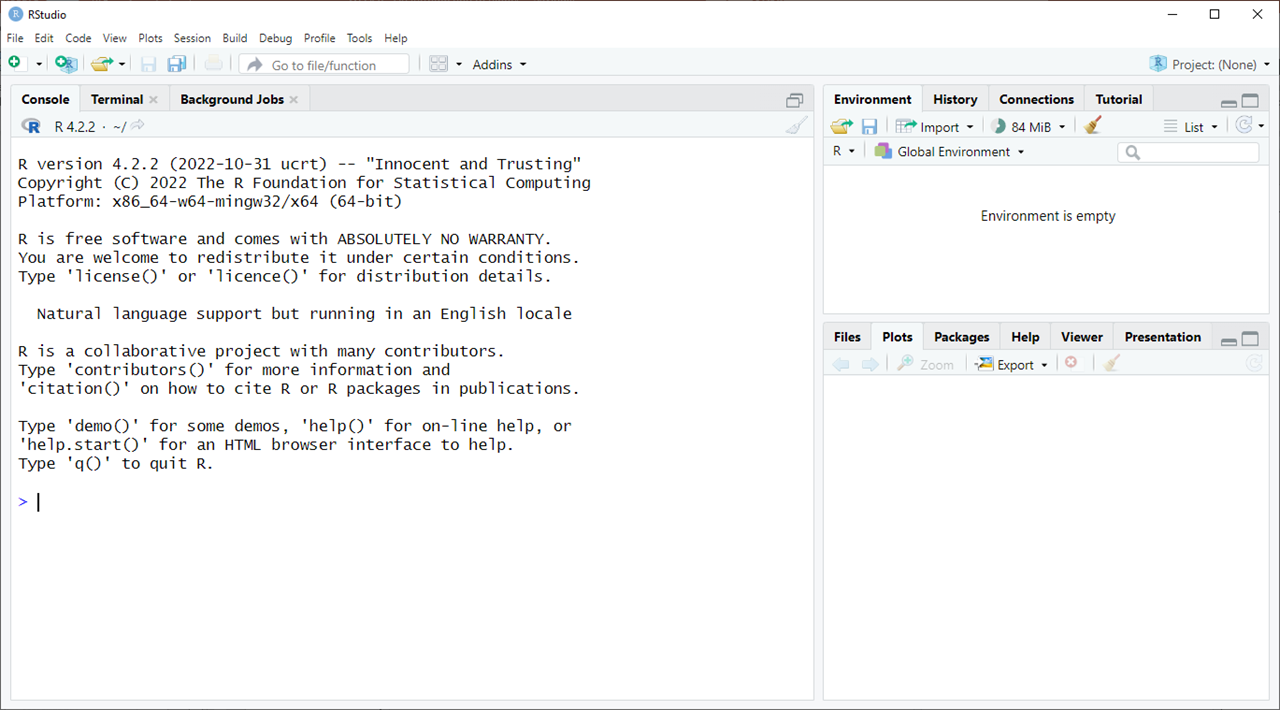
\includegraphics{docs/_main_files/figure-html/RStudio clean install.png}

If your screen looks like the image below, it means that you've accidentally opened RGui, a basic graphical user interface included with \texttt{R}, and not RStudio. We're always going to be working in RStudio for this class, so close out of RGui and open RStudio instead.

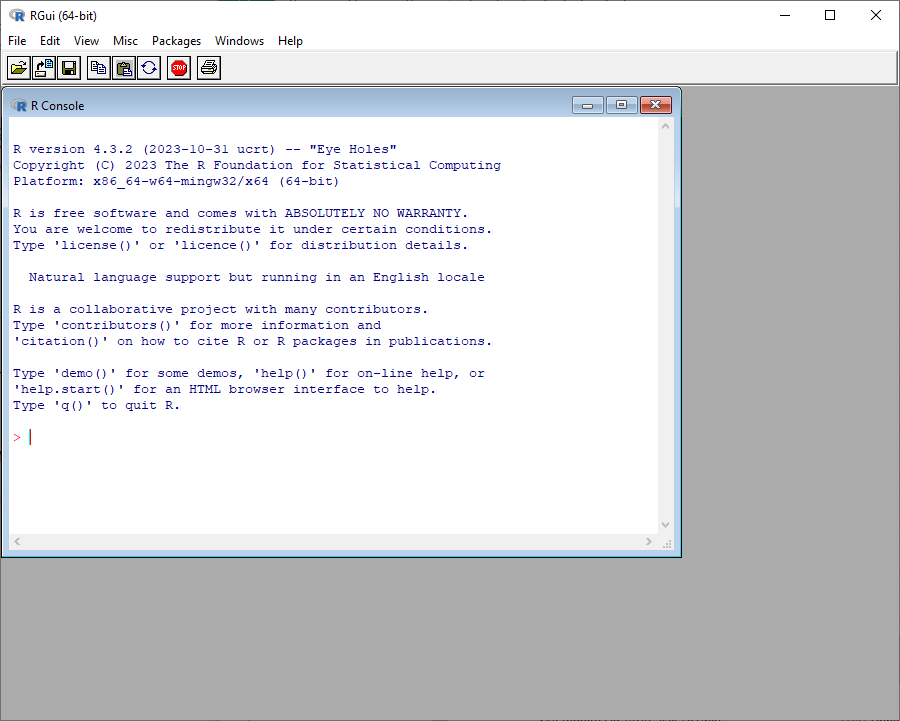
\includegraphics{docs/_main_files/figure-html/Base R GUI.PNG}

\hypertarget{using-the-console}{%
\section{Using the Console}\label{using-the-console}}

Now the fun begins. The RStudio window you've opened consists of a few different parts. The most important of these right now is the console \href{https://docs.posit.co/ide/user/ide/guide/ui/ui-panes.html}{pane} (highlighted below).

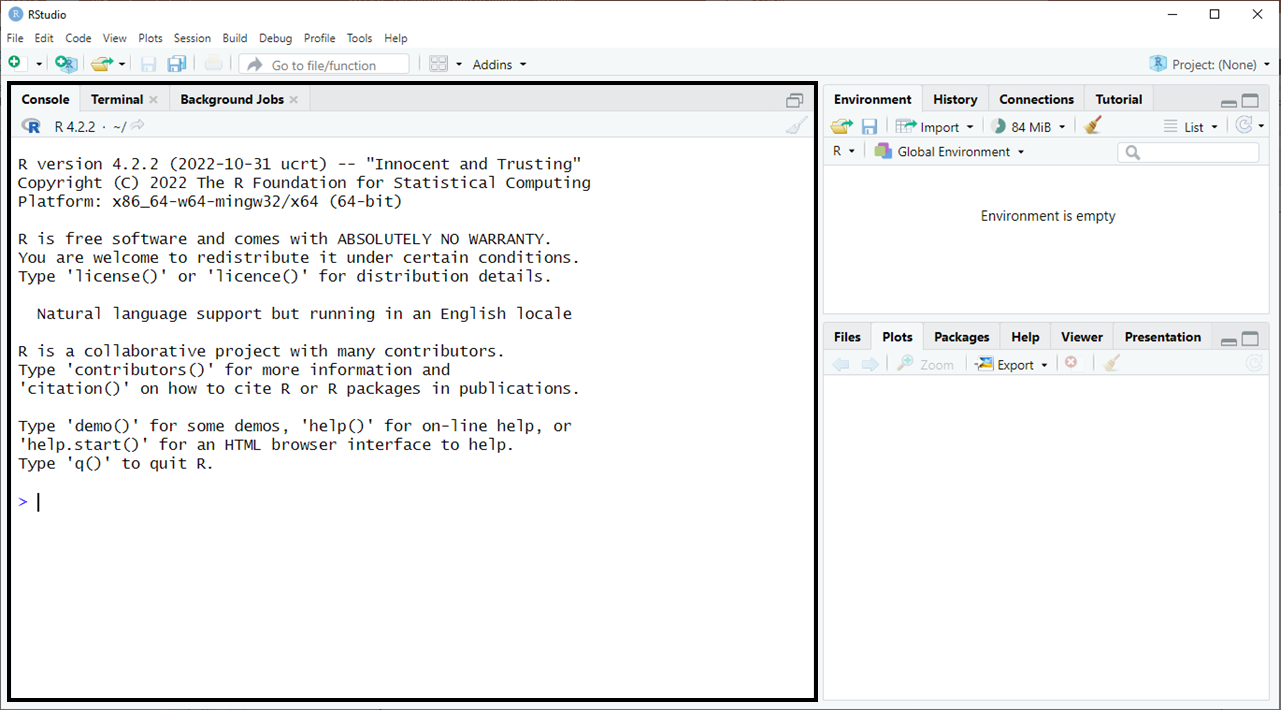
\includegraphics{docs/_main_files/figure-html/RStudio console box.png}

The console allows you to interact with your computer using \texttt{R}. So, for example, if I want to use my computer as an over-sized calculator, I can type in the following \texttt{R} code in the console:

\begin{Shaded}
\begin{Highlighting}[]
\DecValTok{1}\SpecialCharTok{+}\DecValTok{1}
\end{Highlighting}
\end{Shaded}

What happens when you press \texttt{Enter} on your keyboard? You get something like this:

\begin{Shaded}
\begin{Highlighting}[]
\DecValTok{1}\SpecialCharTok{+}\DecValTok{1}
\end{Highlighting}
\end{Shaded}

\begin{verbatim}
## [1] 2
\end{verbatim}

You've provided an \textbf{input}, \texttt{1+1}, and received an \textbf{output}, \texttt{2}. In other words, using the language of \texttt{R}, you've told your computer to add one plus one and your computer has correctly interpreted your command and returned an answer, two. When your computer does not know how to interpret a command, usually because you've made a mistake, you will receive an error message as the output instead. Identifying errors and being able to correct them is an essential skill for a programmer.

One more note about outputs: the first number in brackets next to your output, \texttt{{[}1{]}}, indicates the number of the line of output. This is especially helpful when you are running code that generates multiple lines of output. We will see some examples of this later on.

For now, try entering a few more inputs, such as:

\begin{enumerate}
\def\labelenumi{\arabic{enumi}.}
\item
  \texttt{10/3}
\item
  \texttt{(10/3)\ +\ 1}
\item
  \texttt{(10/3)\ +\ 1\ +\ (5.111)\textbackslash{}\^{}2}
\end{enumerate}

\texttt{R} is able to handle basic math operations with ease. What about other operations? Can you work with variables in \texttt{R}?

Try typing this in the console:

\begin{Shaded}
\begin{Highlighting}[]
\NormalTok{x }\OtherTok{=} \DecValTok{1}
\end{Highlighting}
\end{Shaded}

What happens when you press \texttt{Enter}?

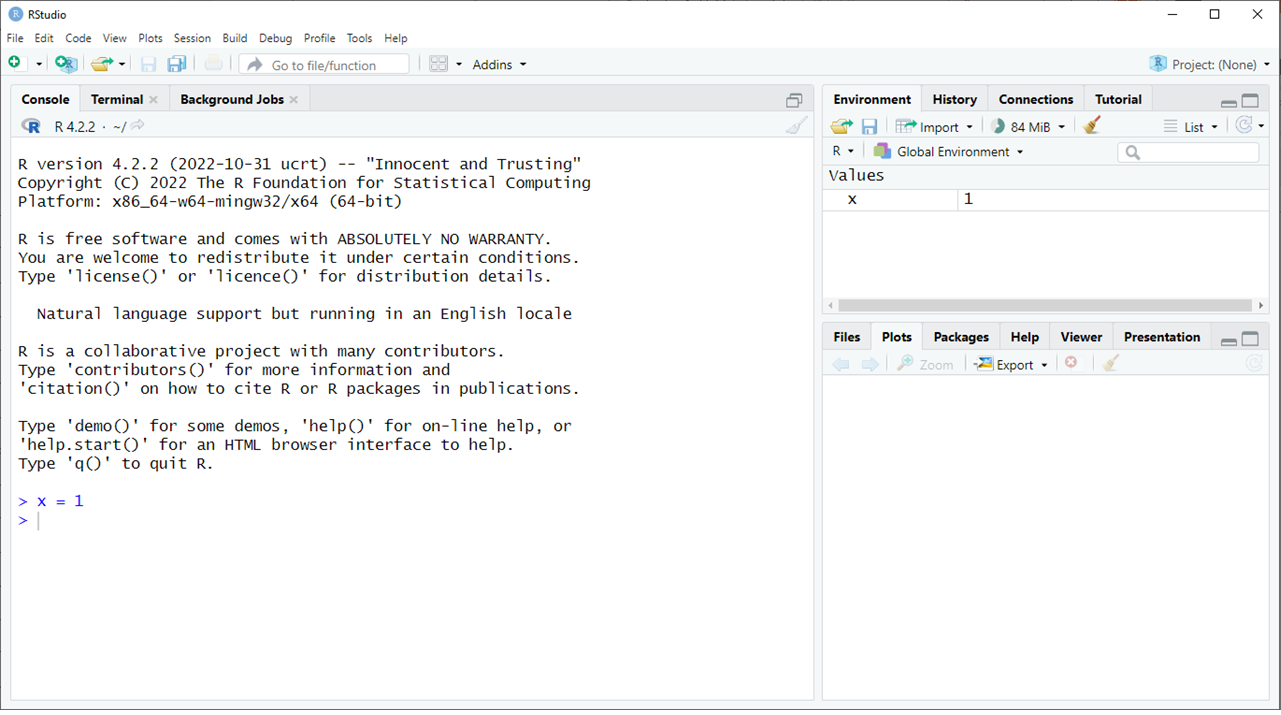
\includegraphics{docs/_main_files/figure-html/RStudio console_x1.png}

You may have noticed that there is no output. But, that doesn't mean nothing has happened. In fact, something has happened. You've stored a value, \texttt{1}, in a variable, \texttt{x}, somewhere in your computer's memory or in what we might call the environment. You don't receive an output, but RStudio reminds you of your new variable's existence via the Environment pane in the top right.

We can recall the value we input into our variable, \texttt{x}, by entering the variable name in the console:

\begin{Shaded}
\begin{Highlighting}[]
\NormalTok{x}
\end{Highlighting}
\end{Shaded}

\begin{verbatim}
## [1] 1
\end{verbatim}

See! Your computer remembers what you stored in your environment.

Try the following:

\begin{enumerate}
\def\labelenumi{\arabic{enumi}.}
\item
  Can you assign a new value to your variable x?
\item
  Can you perform math operations on a variable (e.g., x*2)?
\item
  Can you create a new variable, y, and use it in math operations with x (e.g., x * y)?
\item
  Can you change the type of variable? What if, for example, I don't want x = 1, but I want x equal to the word ``apple''?
\end{enumerate}

\hypertarget{calculations-with-variables}{%
\section{Calculations with Variables}\label{calculations-with-variables}}

If you've made it this far, well done! Here's another thing you can try. Enter the following in the console:

\begin{Shaded}
\begin{Highlighting}[]
\NormalTok{x }\OtherTok{\textless{}{-}} \FunctionTok{c}\NormalTok{(}\DecValTok{1}\NormalTok{,}\DecValTok{2}\NormalTok{,}\DecValTok{3}\NormalTok{,}\DecValTok{4}\NormalTok{,}\DecValTok{5}\NormalTok{)}
\end{Highlighting}
\end{Shaded}

You'll notice that we're using a different operator here. It's a less than symbol (\textless) followed by a dash (-). This is called an \textbf{assignment operator} and it has the same function as the equals sign (=). You can use either, I just so happen to prefer the way this one looks.

What happens when you press \texttt{Enter}? You have created a \textbf{vector}. Like other types of variables in \texttt{R}, a vector is an \textbf{object}. A vector holds a set of values of the same type. In this case, the object x contains a set of numbers, 1:5.

We can do all sorts of things with vectors and other objects in \texttt{R}. We can, for example, find the sum of a vector.

\begin{Shaded}
\begin{Highlighting}[]
\FunctionTok{sum}\NormalTok{(x)}
\end{Highlighting}
\end{Shaded}

\begin{verbatim}
## [1] 15
\end{verbatim}

How did we get an output of 15? 1+2+3+4+5 = 15. We can also find the mean of a vector.

\begin{Shaded}
\begin{Highlighting}[]
\FunctionTok{mean}\NormalTok{(x)}
\end{Highlighting}
\end{Shaded}

\begin{verbatim}
## [1] 3
\end{verbatim}

And, we can perform other fun operations. Try the following:

\begin{enumerate}
\def\labelenumi{\arabic{enumi}.}
\item
  Can you find the median of the vector x? What about the mode?\footnote{As you will have found, \texttt{mode()} doesn't calculate a statistic here (although even if it had, you still wouldn't have gotten a meaningful statistic for this particular vector). Some functions are easy to guess, like \texttt{median()} , but others can be false cognates just like in a spoken language. We'll talk more about finding the purpose of a function in the next chapter.}
\item
  What happens when you multiply a vector?
\item
  Can you create a new vector which consists of a set of letters?
\end{enumerate}

\hypertarget{saving-your-work}{%
\section{Saving Your Work}\label{saving-your-work}}

As you've started to see, working with a scripting language like \texttt{R} is quite different from working with software like Microsoft Excel or Google Sheets. You work interactively with data using code rather than by changing values directly in a user interface. No more clicking on cells to change values, now you change them programmatically.

One of the great advantages of interacting with data in this way, particularly for the social sciences, is that it allows us to see all of the steps you've taken to produce your analysis and repeat them. We don't have to take your word for how you've calculated something. We can see it and use it ourselves to produce the same thing.

This means that we leave our source data alone and write the code that produces the analysis. As with any good recipe, we want the code you write to be clear and easy to follow so that we can come back to it and understand what we did. We'll say more about how to do this later on.

There are a couple of different ways of saving your code:

\begin{enumerate}
\def\labelenumi{\arabic{enumi}.}
\item
  In an R Script, a simple text file ending in a \texttt{.r} extension
\item
  In an R Markdown file, an interactive format that allows you to see your code and the results together in the same file
\end{enumerate}

We're going to start with an R Script file and try out R Markdown later on.

\hypertarget{creating-and-saving-an-r-script}{%
\section{Creating and Saving an R Script}\label{creating-and-saving-an-r-script}}

To create an R Script file in RStudio, go to File \textgreater{} New File \textgreater{} R Script.

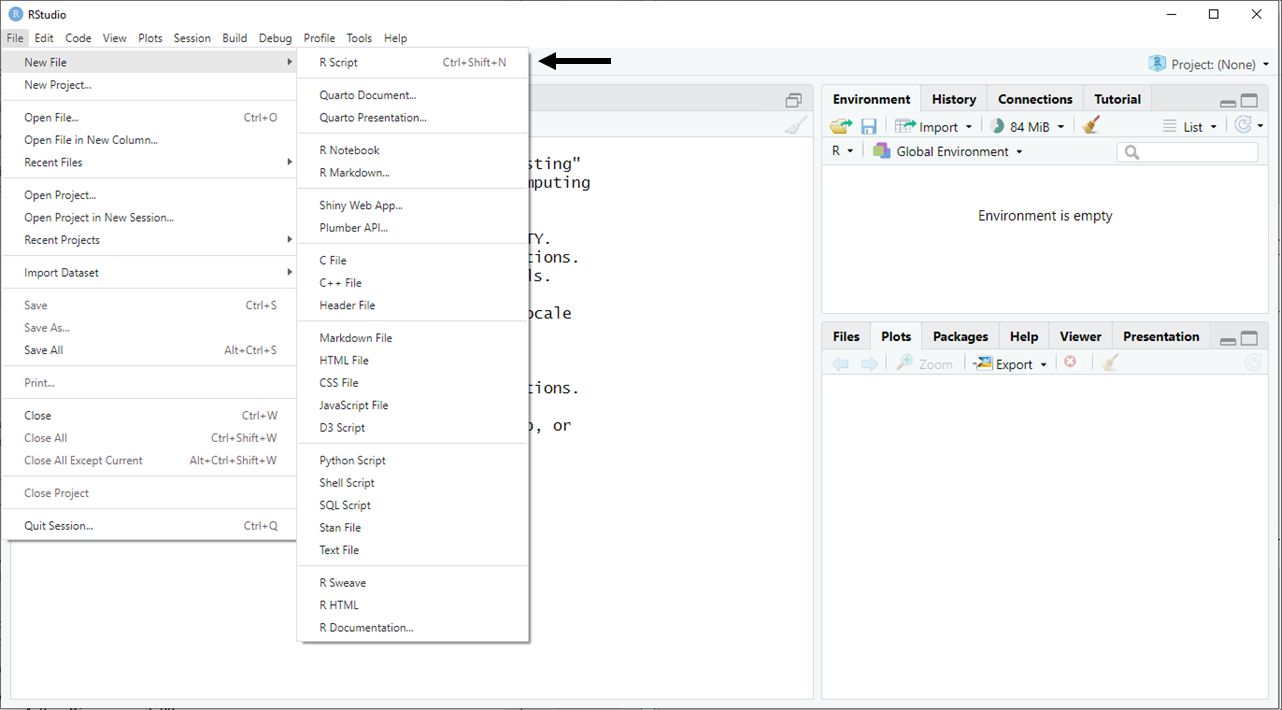
\includegraphics{docs/_main_files/figure-html/RStudio_Opening an R Script File.png}

You should now have a window open in RStudio which looks like this:

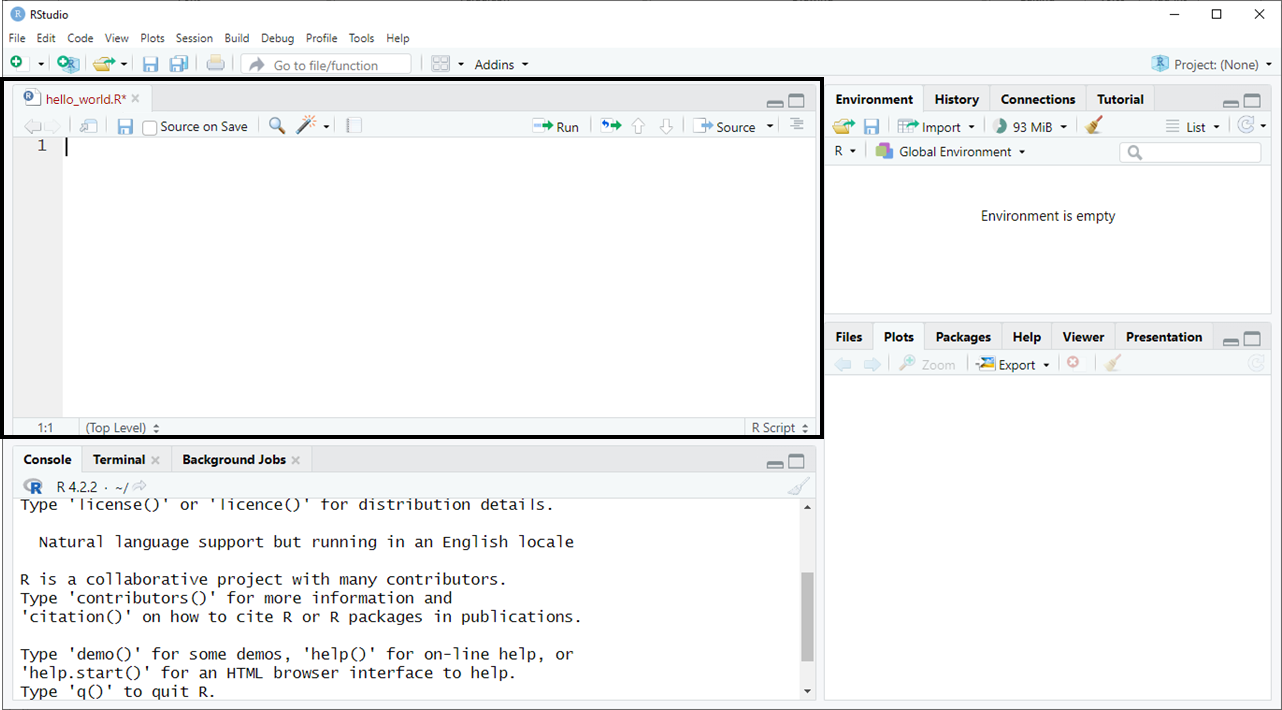
\includegraphics{docs/_main_files/figure-html/RStudio_Opened RScript.png}

You can enter comments in your R Script file using a hash tag (\texttt{\#}) at the beginning of each comment line. A hash tag lets \texttt{R} know that this line should not be run as code. Its purpose is to tell us what is happening in a particular section of the code.

I like to start by adding my name, the date, and a description to each file I use. I'll ask that you use a header for each \texttt{R} file you submit for this class as well.

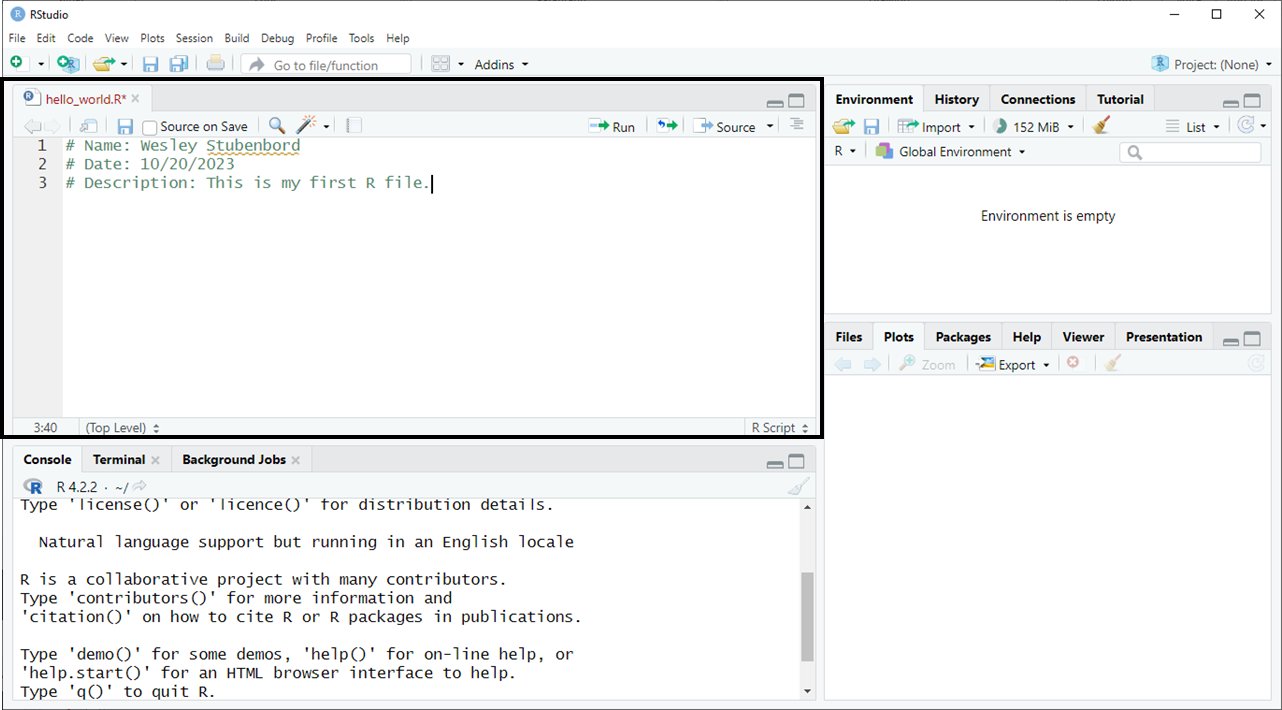
\includegraphics{docs/_main_files/figure-html/RStudio_Commenting in an R Script file.png}

Now, save your R Script somewhere on your computer. Go to File \textgreater{} Save As, then choose a safe place on your computer to store it (I recommend creating a folder for this course), give your file a name, and press save. I called mine ``hello\_world''.

\hypertarget{interacting-in-an-r-script}{%
\section{Interacting in an R Script}\label{interacting-in-an-r-script}}

Interacting in an R Script is slightly different from interacting with the console. Now when you type in code and hit \texttt{Enter}, it will not execute the code, it just creates a new line in your file.

To run code in a script in RStudio, you can either:

\begin{enumerate}
\def\labelenumi{\arabic{enumi}.}
\tightlist
\item
  Select the lines you wish to run with your cursor and then press \texttt{Ctrl} + \texttt{Enter}
\item
  Or, put your cursor on the line you wish to run and click the \texttt{Run} button in the upper-right of the R Script pane
\end{enumerate}

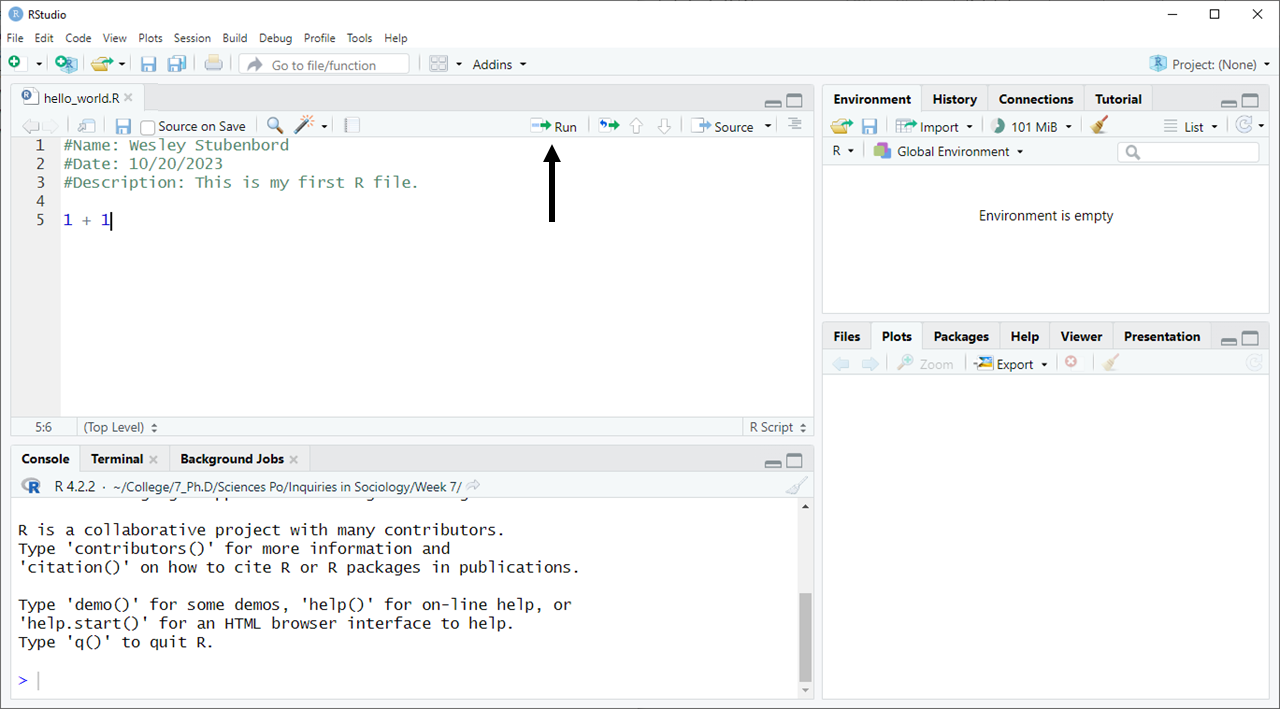
\includegraphics{docs/_main_files/figure-html/RStudio_Run button.png}

The first option allows you to run multiple lines at a time. The second runs only the line you are currently on. The results of your code will appear in the console pane below your R Script file when run successfully.

After you finish modifying your R Script file, you can save it and close out of RStudio. The next time you wish to access your saved code, you can open your R Script file and it will be exactly as you left it.

\hypertarget{summary}{%
\section{Summary}\label{summary}}

Let's briefly recap what you have learned in this lesson. So far you've learned:

\begin{itemize}
\tightlist
\item
  The difference between \texttt{R} and RStudio
\item
  How to interact with the console
\item
  How to create and store values in variables using an assignment operator
\item
  What a vector is and how to create one
\item
  How to use basic functions like \texttt{sum()} and \texttt{mean()} to perform calculations
\item
  How to make comments using the \texttt{\#} symbol
\item
  How to create and save R Script files
\end{itemize}

\hypertarget{working-with-data-in-r}{%
\chapter{\texorpdfstring{Working with Data in \texttt{R}}{Working with Data in R}}\label{working-with-data-in-r}}

Before we can get to the nitty-gritty of working with real data, we need to familiarize ourselves with a few more essential concepts.

\hypertarget{functions}{%
\section{Functions}\label{functions}}

Last class, we assigned a vector to a variable like this:

\begin{Shaded}
\begin{Highlighting}[]
\NormalTok{my\_vector }\OtherTok{\textless{}{-}} \FunctionTok{c}\NormalTok{(}\DecValTok{1}\NormalTok{,}\DecValTok{2}\NormalTok{,}\DecValTok{3}\NormalTok{,}\DecValTok{4}\NormalTok{,}\DecValTok{5}\NormalTok{,}\DecValTok{6}\NormalTok{)}
\end{Highlighting}
\end{Shaded}

Where \texttt{my\_vector} is an object and \({1,2,3,4,5,6}\) is the set of values assigned to it. When you run this code in your console (or in a script file), your new variable and its assigned values are stored in short-term memory and appear in the Environment pane of RStudio.

When we assigned a single value to another variable, however, as in:

\begin{Shaded}
\begin{Highlighting}[]
\NormalTok{x }\OtherTok{\textless{}{-}} \DecValTok{1}
\end{Highlighting}
\end{Shaded}

or,

\begin{Shaded}
\begin{Highlighting}[]
\NormalTok{first\_name }\OtherTok{=} \StringTok{\textquotesingle{}Wesley\textquotesingle{}}
\end{Highlighting}
\end{Shaded}

we didn't use \texttt{c()}. So, what exactly is \texttt{c()}?

Like \texttt{sum()} or \texttt{mean()}, \texttt{c()} is a \textbf{function}. Functions play an important role in all programming languages. They are snippets of code, often hidden in the background, that allow us to accomplish specific tasks, like adding up all of the numbers in a vector, taking the mean, or creating a vector. In \texttt{R}, \texttt{c()} is a function which \textbf{\emph{c}}ombines values into a vector or list.

Functions give us the ability to recall previously written code to perform the same task over again. Why re-write code every time you need to use it, after all, when you could use the same code you used last time? Instead of copying and pasting code, we can put it in a function, save it somewhere, and call it when we need it.

\hypertarget{calling-a-function}{%
\subsection{Calling a Function}\label{calling-a-function}}

When we want to use a function, or `call it' as we will sometimes say, we type in the name of the function, enclose \textbf{arguments} in a set of parentheses, and run the command. The general form looks something like this:

\begin{Shaded}
\begin{Highlighting}[]
\ControlFlowTok{function}\NormalTok{([arg1], [arg2], ...)}
\end{Highlighting}
\end{Shaded}

\hypertarget{using-arguments-in-a-function}{%
\subsection{Using Arguments in a Function}\label{using-arguments-in-a-function}}

In some cases, you may just have one argument for a function, as when you want to use the \texttt{sum()} function to add the elements of a vector:

\begin{Shaded}
\begin{Highlighting}[]
\FunctionTok{sum}\NormalTok{(my\_vector)}
\end{Highlighting}
\end{Shaded}

\begin{verbatim}
## [1] 21
\end{verbatim}

In other cases, you can have multiple arguments:

\begin{Shaded}
\begin{Highlighting}[]
\FunctionTok{sum}\NormalTok{(my\_vector, my\_vector)}
\end{Highlighting}
\end{Shaded}

\begin{verbatim}
## [1] 42
\end{verbatim}

Arguments can be required or optional and the number of arguments and the order in which they are input depends on the specific function you are using and what you are trying to accomplish. The \texttt{sum()} function, for instance, returns the sum of all values given as arguments.

Arguments can also be used to specify options for a function. Take a look at the example below:

\begin{Shaded}
\begin{Highlighting}[]
\FunctionTok{sum}\NormalTok{(my\_vector, }\ConstantTok{NA}\NormalTok{, my\_vector)}
\end{Highlighting}
\end{Shaded}

\begin{verbatim}
## [1] NA
\end{verbatim}

Here we are using the \texttt{sum()} function to add \texttt{my\_vector} twice, as in the previous example, but now with a missing value (\texttt{NA}). Because the sum of two vectors plus a missing value is unknown, we get an unknown value (\texttt{NA}) as the output.

If we want the \texttt{sum()} function to ignore the unknown value, we can provide it with an additional, named argument which tells it to ignore \texttt{NA}. We can specify this by adding \texttt{,\ na.rm\ =\ TRUE} to our function call. See what happens below:

\begin{Shaded}
\begin{Highlighting}[]
\FunctionTok{sum}\NormalTok{(my\_vector, }\ConstantTok{NA}\NormalTok{, my\_vector, }\AttributeTok{na.rm =} \ConstantTok{TRUE}\NormalTok{)}
\end{Highlighting}
\end{Shaded}

\begin{verbatim}
## [1] 42
\end{verbatim}

We're back to an answer of 42. The \texttt{sum()} function ignored the missing value, as we specified, and added the two vectors.

All functions have named arguments and an ordering to them. If you omit the name of an argument in your function call, the function processes them according to their default order. It is generally a good habit to specify argument names, as in the example below where the `x' argument takes the object you are trying to sum, but it is not entirely necessary for simple functions.

\begin{Shaded}
\begin{Highlighting}[]
\FunctionTok{sum}\NormalTok{(}\AttributeTok{x =}\NormalTok{ my\_vector)}
\end{Highlighting}
\end{Shaded}

\begin{verbatim}
## [1] 21
\end{verbatim}

\hypertarget{getting-help-with-functions}{%
\subsection{Getting Help with Functions}\label{getting-help-with-functions}}

As you progress in \texttt{R}, you will learn many different functions and it can be difficult to keep track of all of the different arguments. Whenever you want to know more about what a function does or what arguments it takes, simply type \texttt{?function\_name} into the RStudio console and you will get some useful documentation in the Help pane located in the lower-right of your RStudio window.

\begin{verbatim}
?sum
\end{verbatim}

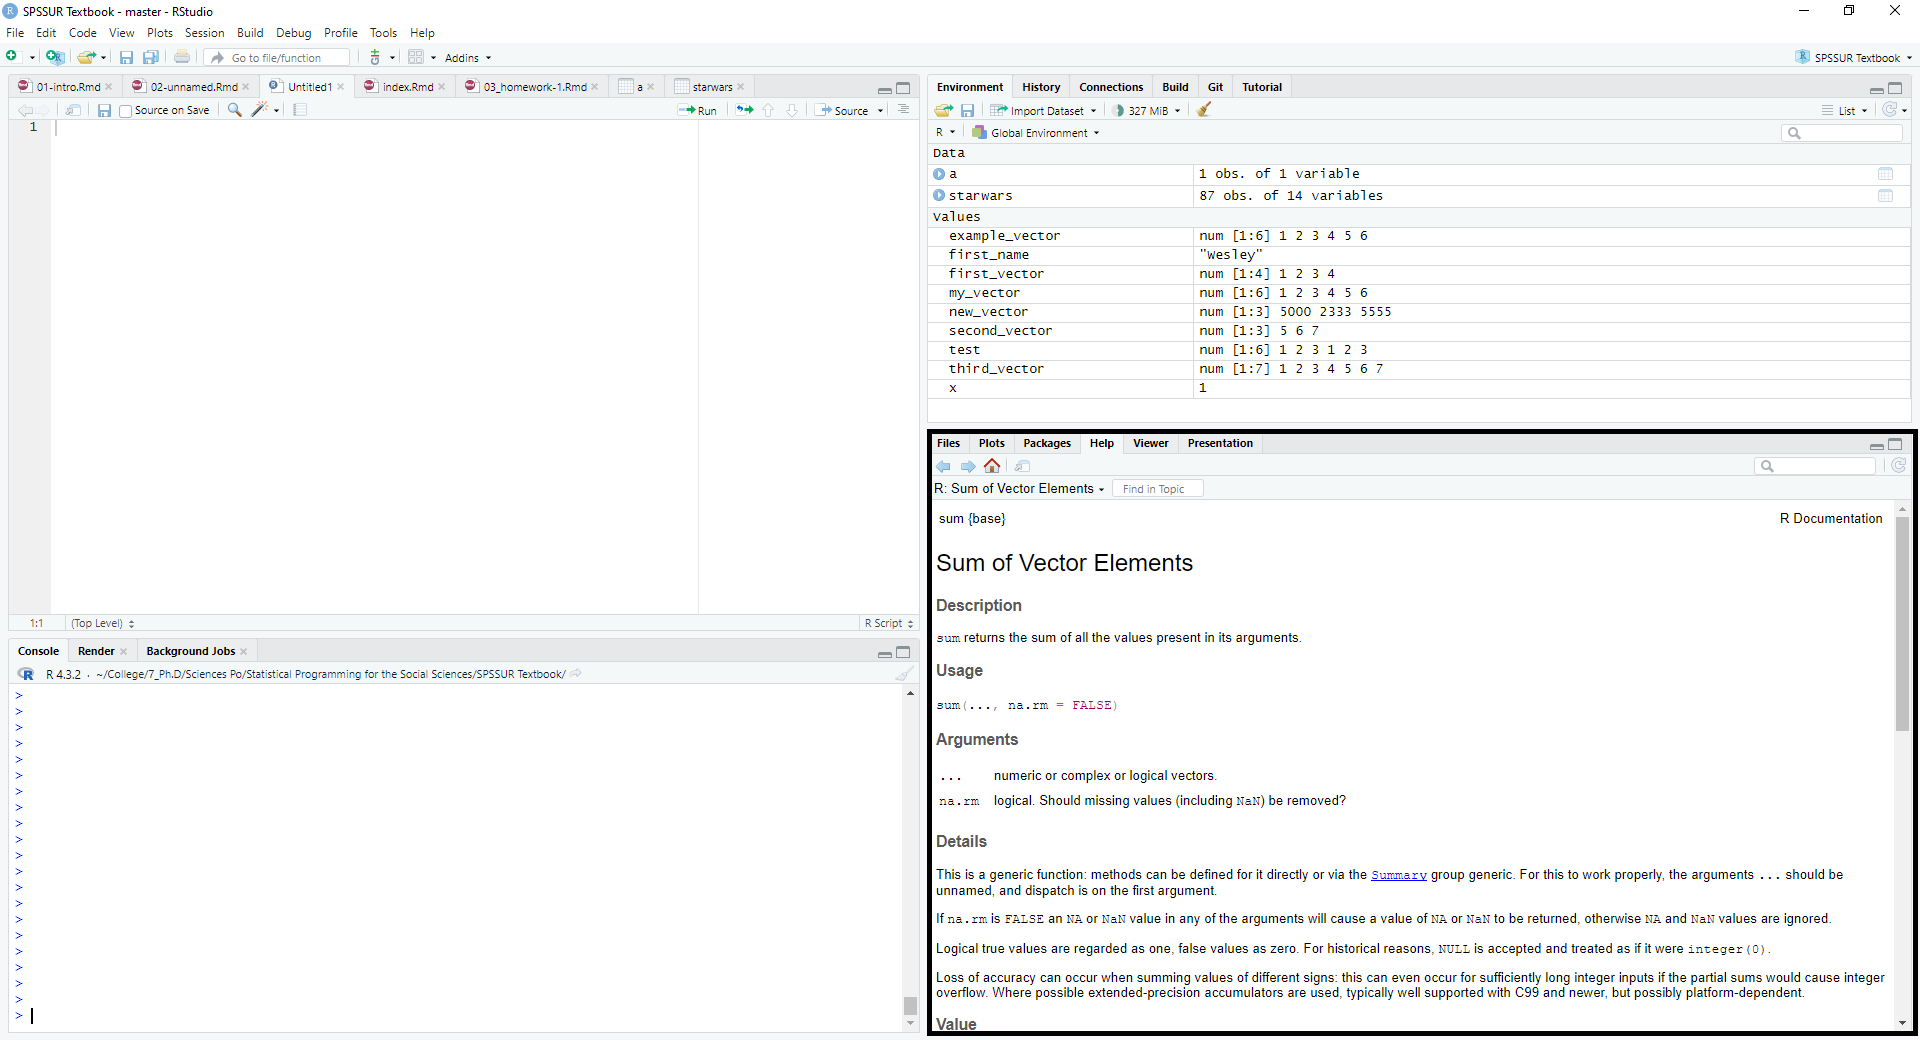
\includegraphics{docs/_main_files/figure-html/RStudio_Help Pane.PNG}

\hypertarget{check-your-understanding}{%
\subsection*{Check Your Understanding:}\label{check-your-understanding}}
\addcontentsline{toc}{subsection}{Check Your Understanding:}

Let's take a quick pause to make sure we understand what we just learned.

\begin{enumerate}
\def\labelenumi{\arabic{enumi}.}
\tightlist
\item
  Create a vector of three numbers and assign it to a variable called \texttt{first\_vector}. Now use the \texttt{mean()} function to find the average of \texttt{first\_vector}.
\item
  Using the \texttt{c()} function, create another vector called \texttt{second\_vector} which includes the values of \texttt{first\_vector} and an \texttt{NA} value. Try it on your own first, then click this footnote to see the answer.\footnote{\texttt{second\_vector\ \textless{}-\ c(first\_vector,\ NA)}}
\item
  Using the \texttt{na.rm\ =\ TRUE} argument, calculate the mean of \texttt{second\_vector}.
\end{enumerate}

\hypertarget{packages}{%
\section{Packages}\label{packages}}

One of the great benefits of \texttt{R} is its power and flexibility. We've seen how functions provide us with the ability to reuse code, but functions are common to any programming language or statistical software.

It may sound cliché, but what makes \texttt{R} special is its community. \texttt{R} is a free and open-source software, which means that anyone can use or contribute to it. If you develop a new statistical method, for instance, you can write the code necessary to implement it and share it with others.

Base \texttt{R}, which you installed last class, comes with a number of built-in functions like \texttt{mean()}, \texttt{sum()}, \texttt{range()}, and \texttt{var()} . But, \texttt{R} users working out of the goodness of their hearts have developed many other functions that accomplish an array of tasks, from making aesthetically-pleasing visualizations to executing complex machine learning algorithms.

These functions are put together into what are called \textbf{packages}, which can be easily installed and loaded into \texttt{R}. Packages can also contain data and other compiled code.

\hypertarget{installing-packages}{%
\subsection{Installing Packages}\label{installing-packages}}

We're going to use the \texttt{install.packages()} function to install one such package, called \textbf{tidyverse}.

\begin{verbatim}
install.packages('tidyverse')
\end{verbatim}

Once you've run this command in your RStudio console, you will have downloaded the tidyverse and saved it to your \textbf{library}. The library is simply where your packages are stored.

\href{https://tidyverse.tidyverse.org/}{Tidyverse} is actually a set of packages, including \texttt{dplyr} and \texttt{ggplot2}, all of which are useful for data analysis in \texttt{R}. We'll be using the tidyverse throughout this course and you will find that it's the most commonly used set of packages for data analysis in \texttt{R}.

\hypertarget{loading-libraries}{%
\subsection{Loading Libraries}\label{loading-libraries}}

Whenever you start an \texttt{R} session and want to use a package, you have to be sure to load it. Loading a package makes sure that your computer knows what functions and data are inside, so that you can call them at will.

To load an \texttt{R} package, you can use the \texttt{library()} function, like this:

\begin{Shaded}
\begin{Highlighting}[]
\FunctionTok{library}\NormalTok{(tidyverse)}
\end{Highlighting}
\end{Shaded}

\begin{verbatim}
## -- Attaching core tidyverse packages ------------------------ tidyverse 2.0.0 --
## v dplyr     1.1.4     v readr     2.1.5
## v forcats   1.0.0     v stringr   1.5.1
## v ggplot2   3.4.4     v tibble    3.2.1
## v lubridate 1.9.3     v tidyr     1.3.1
## v purrr     1.0.2     
## -- Conflicts ------------------------------------------ tidyverse_conflicts() --
## x dplyr::filter() masks stats::filter()
## x dplyr::lag()    masks stats::lag()
## i Use the conflicted package (<http://conflicted.r-lib.org/>) to force all conflicts to become errors
\end{verbatim}

Now, that you've loaded tidyverse, you can access it's special functions like \texttt{mutate()} or its data sets, like \texttt{starwars}. Try entering \texttt{starwars} in your console after you've loaded the tidyverse. What's inside?

\hypertarget{loading-data}{%
\section{Loading Data}\label{loading-data}}

Great, you know what a function is, you have the tidyverse installed, and you've seen that data can be contained in packages, which are easy to install and load.

\hypertarget{using-data-from-packages}{%
\subsection{Using Data from Packages}\label{using-data-from-packages}}

Let's install and load another package, so that we can take a look at some more data.

\begin{verbatim}
install.packages('socviz')
\end{verbatim}

\begin{Shaded}
\begin{Highlighting}[]
\FunctionTok{library}\NormalTok{(socviz)}
\end{Highlighting}
\end{Shaded}

The \texttt{socviz} package accompanies a textbook called \textbf{\emph{Data Visualization}} written by Kieran Healy, a Professor of Sociology at Duke University, and it contains some interesting datasets including election data from the 2016 U.S. presidential election. This dataset is stored in an object titled \texttt{election}. Once you have \texttt{socviz} installed and loaded, you can get a preview of its contents by entering the name of the object:

\begin{Shaded}
\begin{Highlighting}[]
\NormalTok{election}
\end{Highlighting}
\end{Shaded}

\begin{verbatim}
## # A tibble: 51 x 22
##    state     st     fips total_vote vote_margin winner party pct_margin r_points
##    <chr>     <chr> <dbl>      <dbl>       <dbl> <chr>  <chr>      <dbl>    <dbl>
##  1 Alabama   AL        1    2123372      588708 Trump  Repu~     0.277     27.7 
##  2 Alaska    AK        2     318608       46933 Trump  Repu~     0.147     14.7 
##  3 Arizona   AZ        4    2604657       91234 Trump  Repu~     0.035      3.5 
##  4 Arkansas  AR        5    1130635      304378 Trump  Repu~     0.269     26.9 
##  5 Californ~ CA        6   14237893     4269978 Clint~ Demo~     0.300    -30.0 
##  6 Colorado  CO        8    2780247      136386 Clint~ Demo~     0.0491    -4.91
##  7 Connecti~ CT        9    1644920      224357 Clint~ Demo~     0.136    -13.6 
##  8 Delaware  DE       10     443814       50476 Clint~ Demo~     0.114    -11.4 
##  9 District~ DC       11     311268      270107 Clint~ Demo~     0.868    -86.8 
## 10 Florida   FL       12    9502747      112911 Trump  Repu~     0.0119     1.19
## # i 41 more rows
## # i 13 more variables: d_points <dbl>, pct_clinton <dbl>, pct_trump <dbl>,
## #   pct_johnson <dbl>, pct_other <dbl>, clinton_vote <dbl>, trump_vote <dbl>,
## #   johnson_vote <dbl>, other_vote <dbl>, ev_dem <dbl>, ev_rep <dbl>,
## #   ev_oth <dbl>, census <chr>
\end{verbatim}

For ease of use, we're going to store a copy of this data in a new object in our environment called \texttt{election\_2016}.

\begin{Shaded}
\begin{Highlighting}[]
\NormalTok{election\_2016 }\OtherTok{\textless{}{-}}\NormalTok{ election}
\end{Highlighting}
\end{Shaded}

Now, we can play around with it. In addition to getting a preview of the data by entering the name of our object in the console, we can also access it through the Environment pane of our RStudio window. Click on \texttt{election\_2016} and you will see the full dataset.

Just like in a spreadsheet, you can scroll through the full set of columns and rows. Remember, of course, that you cannot edit values in this view tab. This is by design. If we want to make changes to the data or perform calculations, we need to do so programmatically.

\hypertarget{data-types-and-data-structures}{%
\section{Data Types and Data Structures}\label{data-types-and-data-structures}}

This seems about as good a point as any to talk about the different types of data you will be working with in R.

\hypertarget{data-types}{%
\subsection{Data Types}\label{data-types}}

There are six different basic data types in \texttt{R}. The most important for our purposes are:

\begin{itemize}
\tightlist
\item
  \textbf{character}: letters such as `a' or sets of letters such as `apple'
\item
  \textbf{numeric}: numbers such as 1, 1.1 or 23
\item
  \textbf{logical}: the boolean values, TRUE and FALSE
\end{itemize}

The other types are integers (which can only hold integers and take the form \texttt{1L}), complex (as in complex numbers with an imaginary component, 1+2i), and raw (raw data in the form of bytes). You have already used the previous three and we will never use the latter three.

If you wish to check the data type of an object, you can use the \texttt{class()} function.

\begin{Shaded}
\begin{Highlighting}[]
\FunctionTok{class}\NormalTok{(my\_vector)}
\end{Highlighting}
\end{Shaded}

\begin{verbatim}
## [1] "numeric"
\end{verbatim}

\hypertarget{data-structures}{%
\subsection{Data Structures}\label{data-structures}}

There are many different data structures in \texttt{R}. You've already become familiar with one, vectors, a set of values of the same type. Other types of data structures include:

\begin{itemize}
\tightlist
\item
  \textbf{list}: a set of values of different types
\item
  \textbf{factor:} an ordered set of values, often used to define categories in categorical variables
\item
  \textbf{data frame}: a two-dimensional table consisting of rows and columns similar to a spreadsheet
\item
  \textbf{tibble:} a special version of a data frame from the \emph{tidyverse}, intended to keep your data nice and tidy
\end{itemize}

Note that data structures are usually subsettable, which means that you can access elements of them. Observe:

\begin{Shaded}
\begin{Highlighting}[]
\NormalTok{my\_list }\OtherTok{\textless{}{-}} \FunctionTok{c}\NormalTok{(}\StringTok{\textquotesingle{}a\textquotesingle{}}\NormalTok{, }\StringTok{\textquotesingle{}b\textquotesingle{}}\NormalTok{, }\StringTok{\textquotesingle{}c\textquotesingle{}}\NormalTok{, }\DecValTok{2}\NormalTok{)}
\NormalTok{my\_list[}\DecValTok{2}\NormalTok{]}
\end{Highlighting}
\end{Shaded}

\begin{verbatim}
## [1] "b"
\end{verbatim}

In the example above, we've called an element of the list, \texttt{my\_list}, using an index number in a set of brackets. Since we entered the index, \texttt{2}, inside brackets next to our list name, we received the second element of the list, the character \texttt{b}. We can also modify elements of a list in the same way.

Let's say that I now want to change `b', the second element of \texttt{my\_list}, to the word `blueberry':

\begin{Shaded}
\begin{Highlighting}[]
\NormalTok{my\_list[}\DecValTok{2}\NormalTok{] }\OtherTok{\textless{}{-}} \StringTok{\textquotesingle{}blueberry\textquotesingle{}}
\NormalTok{my\_list}
\end{Highlighting}
\end{Shaded}

\begin{verbatim}
## [1] "a"         "blueberry" "c"         "2"
\end{verbatim}

Easy enough. Now try it out yourself:

\begin{enumerate}
\def\labelenumi{\arabic{enumi}.}
\tightlist
\item
  Create a vector with three elements: ``sociology'', ``economics'', and ``psychology''
\item
  Call each of them individually.
\item
  Change the value of the second element to the value of the first element.
\item
  Change the value of the third element to the value of the first element.
\end{enumerate}

Be sure to do the last two programmatically rather than by re-typing the initial values.

\hypertarget{using-functions-with-data}{%
\section{Using Functions with Data}\label{using-functions-with-data}}

Back to the elections data. We have our 2016 U.S. Presidential Election data stored in a \textbf{tibble} called \texttt{election\_2016}.

If I want to output a single column from the data, I can do so by typing in the name of the data followed by the \texttt{\$} symbol, also known as the \textbf{subset operator}, and the name of the column.

\begin{Shaded}
\begin{Highlighting}[]
\NormalTok{election\_2016}\SpecialCharTok{$}\NormalTok{state}
\end{Highlighting}
\end{Shaded}

\begin{verbatim}
##  [1] "Alabama"              "Alaska"               "Arizona"             
##  [4] "Arkansas"             "California"           "Colorado"            
##  [7] "Connecticut"          "Delaware"             "District of Columbia"
## [10] "Florida"              "Georgia"              "Hawaii"              
## [13] "Idaho"                "Illinois"             "Indiana"             
## [16] "Iowa"                 "Kansas"               "Kentucky"            
## [19] "Louisiana"            "Maine"                "Maryland"            
## [22] "Massachusetts"        "Michigan"             "Minnesota"           
## [25] "Mississippi"          "Missouri"             "Montana"             
## [28] "Nebraska"             "Nevada"               "New Hampshire"       
## [31] "New Jersey"           "New Mexico"           "New York"            
## [34] "North Carolina"       "North Dakota"         "Ohio"                
## [37] "Oklahoma"             "Oregon"               "Pennsylvania"        
## [40] "Rhode Island"         "South Carolina"       "South Dakota"        
## [43] "Tennessee"            "Texas"                "Utah"                
## [46] "Vermont"              "Virginia"             "Washington"          
## [49] "West Virginia"        "Wisconsin"            "Wyoming"
\end{verbatim}

If I want to perform a calculation on a column, I can pass the column as an argument to a function like so:

\begin{Shaded}
\begin{Highlighting}[]
\CommentTok{\# Sum the total number of votes cast in the 2016 Presidential election.}
\FunctionTok{sum}\NormalTok{(election\_2016}\SpecialCharTok{$}\NormalTok{total\_vote, }\AttributeTok{na.rm =} \ConstantTok{TRUE}\NormalTok{)}
\end{Highlighting}
\end{Shaded}

\begin{verbatim}
## [1] 137125484
\end{verbatim}

The \texttt{na.rm} argument isn't strictly necessary in this case (since there are no missing or unknown values), but it's good to remember that it's there when you need it.

For the remainder of today's session, I'd like you play around with this data. In particular:

\begin{enumerate}
\def\labelenumi{\arabic{enumi}.}
\tightlist
\item
  Identify the variable type for the \texttt{ST}, \texttt{pct\_johnson}, and \texttt{winner} columns.
\item
  Calculate the mean \texttt{vote\_margin} across the states.
\item
  Use the \texttt{table()} function to count the number of states won by each presidential candidate.
\item
  Create a variable which contains the total number of votes received by Hillary Clinton (contained in the column \texttt{clinton\_vote}) and a variable containing the total number of votes received by Donald Trump (\texttt{trump\_vote}). Take the difference of the two.
\item
  Create a variable containing the total number of electoral votes received by Hillary Clinton (contained in \texttt{ev\_dem}) and another containing the total number received by Donald Trump (\texttt{ev\_rep}). Take the difference of the two.
\item
  Try using the \texttt{plot(x=,\ y=)} function to plot a couple of numeric columns.
\end{enumerate}

\hypertarget{homework-1}{%
\chapter*{Homework 1}\label{homework-1}}
\addcontentsline{toc}{chapter}{Homework 1}

\textbf{Due Date:} Sunday, 11 February by 23:59:59

\textbf{Submission Instructions:} Submit your completed R script file to Moodle.

  \bibliography{book.bib,packages.bib}

\end{document}
